%\customHeader{1}{Preprocessing the \VSI{} dataset}
%\label{vsi_preprocessing}



% %%%%%%%%%%%%%%%%%%%%%%%%%%%%%%%%%%%%%%%%%%%%%%%%%%%%%%%%%%%%%%%%%%%%%%%%%%%%%%%%%%%%%%
\customHeader{1}{Leveraging Keywords}
\label{vsi_leveraging_keywords}

Leveraging the available keywords and key phrases used for the Search Engine queries used to construct the dataset (Table \ref{tab:04_query_keywords}), we obtained four more sources of content. 

\begin{figure}
    \centering
    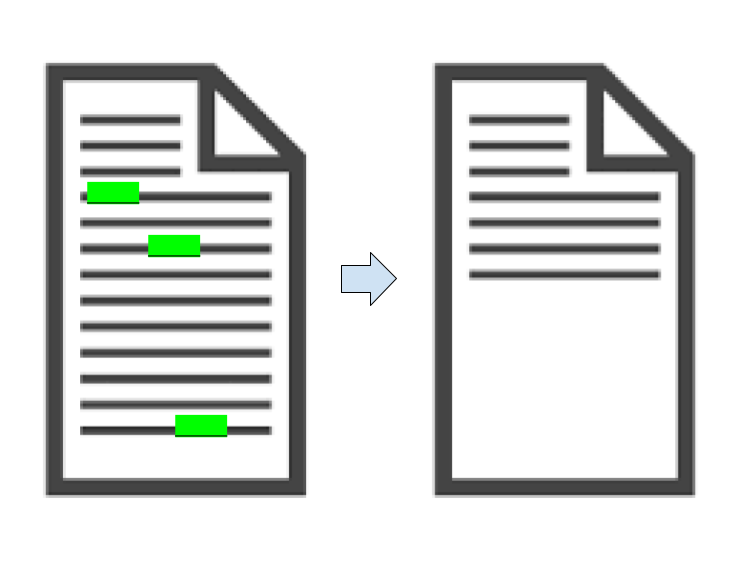
\includegraphics[width=0.5\textwidth]{Figures/05/05_keyphrase_extraction.png}
    \caption{Extracting phrases with Keywords}
    \label{fig:05_keyphrase_extraction}
\end{figure}

%We opted to extract sentences containing keywords or key phrases from the content. 
Using the Python package \texttt{NLTK} \myparencite{nltk}, we divided each document into phrases and selected those containing at least one of the keywords or key phrases. This process was carried out for both the \trafilaturaAbstract{} and \trafilaturaFulltext{} sources of content (Figure \ref{fig:05_keyphrase_extraction}). 
However, considering the diverse range of languages in the documents, it was not always apparent whether we should discard the content entirely or retain it. For example, even if the keyword is not present in the text, maybe its translation is; or we could be facing a language written in a non-Latin script.
Consequently, we pursued two different approaches: in one case, we discarded the original content (O.C.), and in the other, we retained it, resulting in four new sources of content (Table \ref{tab:05_pesv_sources of content after preprocessing}).

\begin{table}%[]
    \centering
    \begin{tabular}{c|c}
       \textbf{\contentType{}}  & \textbf{Tool} \\ \hline
       \trafilaturaTitle{}  & Trafilatura \\
       \trafilaturaAbstract{}  & Trafilatura \\
       \trafilaturaFulltext{}  & Trafilatura \\
       \translationTitle{}  & Google Translate \\
     \keyphrasesAbstractOnly{} & Preprocessing \\
     \keyphrasesAbstractOC{} & Preprocessing \\
     \keyphrasesFulltextOnly{} & Preprocessing \\
     \keyphrasesFulltextOC{} & Preprocessing \\ 
    \end{tabular}
    \caption{Sources of text content in the \VSI{} Dataset after preprocessing}
    \label{tab:05_pesv_sources of content after preprocessing}
\end{table}


Figure \ref{fig:05_unique_entries_keyphrases_vsi} offers a comparison of the number of unique entries per content source. In both cases, keeping only the phrases containing keywords dramatically reduces the size of the data, especially for the \trafilaturaAbstract{}. Possible reasons for this will be explained in \headerName{} \ref{vsi_data_cleaning}. Note that, in the case of keeping the original content, there are slightly fewer unique entries for both the \trafilaturaAbstract{} and the \trafilaturaFulltext{} ($19,939-19,798 = 141$ and $26,346-24,447=1,899$, respectively). This may be explained by the fact that some data noise may be removed by the sentence extraction process, especially those cases where several entries differ by a small amount of tokens (see Table \ref{tab:04_website_names_as_suffixes}).

\begin{figure}
    \centering
    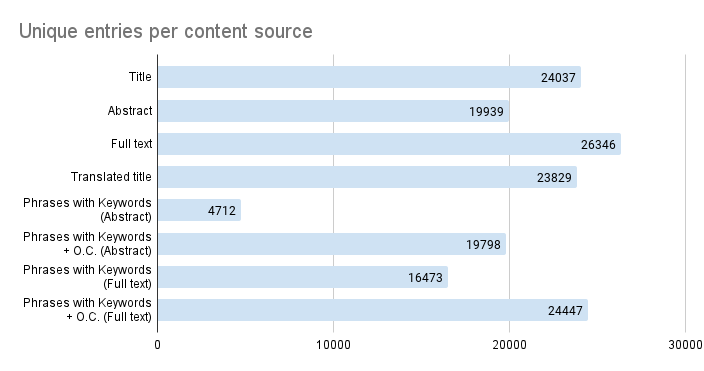
\includegraphics[width=0.750\textwidth]{Figures/05/Unique entries per content source_keyphrases.png}
    \caption{Unique entries per source of content in the \VSI{} dataset}
    \label{fig:05_unique_entries_keyphrases_vsi}
\end{figure}


% %%%%%%%%%%%%%%%%%%%%%%%%%%%%%%%%%%%%%%%%%%%%%%%%%%%%%%%%%%%%%%%%%%%%%%%%%%%%%%%%%%%%%%
\customHeader{1}{Data Cleaning}
\label{vsi_data_cleaning}



\customHeader{2}{Noise Removal}
\label{vsi_string_cleaning}

To address the text noise mentioned in \headerName{} \ref{vsi_issues_data_noise}, we use regular expressions to:

\begin{enumerate}
    \item Remove characters not in any human alphabet. This handles encoding errors.
    \item Remove emojis, URLs, HTML tags, hours, dates, extra white spaces.
    \item Remove punctuation at beginning and end of the string.
    \item Remove digits at beginning and end of the string.
    \item Standardize quotation characters into the ASCII simple quotation character (').
    \item Standardize hyphen-like characters into the ASCII hyphen (-).
    \item Remove sentence suffixes that may be the name of the website, by deleting short text ($\leq 3$ tokens) that follow an ASCII hyphen or bar (|) near the end of the string.
\end{enumerate}

See Table \ref{appendix02:tab:pesv_string_cleaning_regex} in the \appendixname{} for some examples of the regular expressions used to clean the multilingual strings. Figure \ref{fig:05_multilingual_string_cleaning} shows the effect of string cleaning on an example text.

\begin{figure}
    \centering
    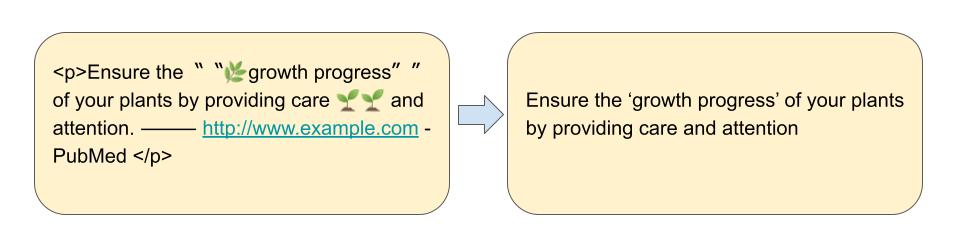
\includegraphics[width=\textwidth]{Figures/05/05_multilingual_string_cleaning.png}
    \caption{Removing noise from multilingual strings}
    \label{fig:05_multilingual_string_cleaning}
\end{figure}


\customHeader{2}{Deleting Error Messages}
\label{vsi_deleting_error_messages}

Fortunately, error messages in the dataset are very consistent. Given that they do not provide information on the relevance of a document, we may delete them using regular expressions. See Table \ref{appendix02:tab:error_messages} in the \appendixname{} for some examples of the regular expressions used to remove the error messages. 

\begin{table}%[]
    \centering
    \begin{tabular}{|lcc|}
    \hline
    \textbf{\contentType{}} & \textbf{Error Count} & \textbf{Percentage of Raw dataset} \\ \hline
    \trafilaturaTitle{} & 7224 & 20.89\% \\
    \trafilaturaAbstract{} & 12624 & 36.50\% \\
    \trafilaturaFulltext{} & 6609 & 19.11\% \\
    \translationTitle{} & 7232 & 20.91\% \\ \hline
    All \contentType{}s & 6399 & 18.50\% \\
    \hline
    \end{tabular}
    \caption{Error Message Count per \contentType{} in the \VSI{} dataset}
    \label{tab:05_vsi_error_message_count}
\end{table}


In Table \ref{tab:05_vsi_error_message_count}, we present the number of error messages identified using our regular expressions. Notably, the proportion of error messages generally hovers around one-fifth of all entries. In $18.50\%\ (\approx 20\%)$ of cases \trafilatura{} completely fails to obtain any content from the website. This proportion almost doubles ($36.50\approx 40\%$) for the \trafilaturaAbstract{}. This discrepancy in the \trafilaturaAbstract{} could be attributed to the common occurrence of missing metadata, as discussed in \headerName{} \ref{vsi_data_statistics}.


\customHeader{2}{Handling scrapping errors}
\label{05_vsi_handling_scrapping_errors}
% first attempt with title names regex. failed ~ 300 docs fewer
% second attempt: by length


In order to handle scraping errors from \trafilatura{}, such as obtaining the name of the website or certain HTML headers, our first approach was to use regular expressions to filter them out. After removing the error messages from all sources of content, we proceeded to count the occurrences of each entry and ranked them in descending order. Given that our dataset contains approximately 35,000 documents, we focused on entries that appeared at least twice.

Although we attempted to identify common patterns and create regular expressions to match frequent entries, this approach proved unsuccessful. It only filtered around 500 unique entries, accounting for a mere $2\%$ of all unique entries in the best case (\trafilaturaAbstract{}). Consequently, it became apparent that several scraping errors likely appeared only once in the dataset, rendering our previous strategy ineffective.

Nevertheless, along this examination, we noticed that scraping errors tend to be short in length (see Tables \ref{tab:04_headers} and \ref{tab:04_website_names}). As a result, we devised a new filtering strategy based on the length of the entries. However, simply counting naive tokens was insufficient, as languages like Chinese often lack whitespace in their text. Therefore, we needed a more robust algorithm to determine when a string is considered suspiciously ``too short."

Our heuristic to filter by length consists in:

\begin{enumerate}
    \item First, the string is split on white spaces.
    \item Then, if there is only one token, and the string has less than 20 characters, it is considered ``too short".
    \item Next, if there are less than four tokens, the string is considered ``too short"
    \item Finally, in all other cases, we keep the string.
\end{enumerate}


\begin{table}%[]
    \centering
    \begin{tabular}{|lcc|}
    \hline
    \textbf{\contentType{}} & \textbf{Short Message Count} & \textbf{Percentage of Raw dataset} \\ \hline
    \trafilaturaTitle{} & 5691 & 16.45\% \\
    \trafilaturaAbstract{} & 1023 & 2.96\% \\
    \trafilaturaFulltext{} & 181 & 0.52\% \\
    \translationTitle{} & 5306 & 15.34\% \\ \hline
    All \contentType{}s & 17 & 0.05\% \\
    \trafilaturaTitle{} $+$ \trafilaturaAbstract{}  & 589   & 1.70\% \\
    \trafilaturaTitle{} $+$ \trafilaturaFulltext{} & 141 & 0.41\% \\
    \trafilaturaFulltext{} $+$ \trafilaturaAbstract{}  & 50   & 0.06\% \\
    \hline
    \end{tabular}
    \caption{Short Message Count per \contentType{} in the \VSI{} dataset}
    \label{tab:05_vsi_short_document_count}
\end{table}


Upon removing error messages, we observed that parsing errors occur in entries for the \trafilaturaTitle{} and the \translationTitle{} approximately 1 in 7 times ($\approx 16\% $), as can be seen in Table \ref{tab:05_vsi_short_document_count}. The \trafilaturaAbstract{} and \trafilaturaFulltext{} are rarely short ($\leq 3\% $), and very few entries have more than one content source that is too brief ($\leq 3\% $).


% %%%%%%%%%%%%%%%%%%%%%%%%%%%%%%%%%%%%%%%%%%%%%%%%%%%%%%%%%%%%%%%%%%%%%%%%%%%%%%%%%%%%%%
\customHeader{1}{Resolving Inconsistencies and Duplicate Documents}
\label{vsi_resolving_inconsistencies}

The initial preprocessing steps focused solely on cleaning the textual content of the dataset. Now, our attention turns to addressing the labeling challenges, specifically, instances where entries have identical content but differ in subject assignment or lack a subject (as in Tables \ref{tab:04_xmol_inconsistencies} and \ref{tab:04_annotation_inconsistencies}).

Considering our main goal is to automate the identification of articles relevant to the \gls{vsi} experts, where subject assignment signifies their interest, we propose the following strategy:

\putInBox{
For each of the eight content sources, we group the dataset based on the text content. If a particular text has been assigned a subject at least once, we categorize it as \textbf{relevant}. Conversely, if no subject has been assigned to a text, we consider it \textbf{irrelevant}.
}

We believe this strategy reflects the intention of the annotators as they labeled the documents (see \headerName{} \ref{vsi_data_annotation}). Additionally, by design, this strategy eliminates duplicate content. Table \ref{tab:determining_relevance} illustrates this process for the content from the \trafilaturaTitle{}.

\begin{table}
    \centering
    \resizebox{0.75\textwidth}{!}{
    \begin{tabular}{cp{10cm}c}
    \textbf{Entry ID} & \textbf{\trafilaturaTitle{}} & \textbf{Subject} \\ \hline
    4662 & Cousin of crop-killing bacteria mutating rapidly & None \\
    5885 & Cousin of crop-killing bacteria mutating rapidly & 4472 \\ \hline
    19661 & Modeling climate change impacts on potential  \ldots & None\\
    19361 & Modeling climate change impacts on potential \ldots - PubMed & None\\ \hline
    58 & Danger pour les végétaux : première détection de \ldots & None \\
    850 & Danger pour les végétaux : première détection de \ldots & 4259 \\ \hline
    26873 & Commodity risk assessment of ash logs from the US \ldots & 5524 \\
    27196 & Commodity risk assessment of ash logs from the US \ldots & 5530 \\ \hline
    29896 & Tornano le Giornate Fai di Primavera \ldots & None  \\
    29899 & Tornano le Giornate Fai di Primavera \ldots - LegnanoNews & None \\\hline
    \vdots & \vdots & \vdots

    \end{tabular} 
    }
    \vspace{0.25cm}
    \begin{center}
       \huge{$\Downarrow$}
    \end{center}
    \vspace{0.25cm}

    \centering
    \resizebox{0.75\textwidth}{!}{
    \begin{tabular}{p{10cm}c}
    
    \textbf{\trafilaturaTitle{}} & \textbf{Relevance} \\ \hline
    Cousin of crop-killing bacteria mutating rapidly & $1$ \\ \hline
    Modeling climate change impacts on potential  \ldots & $0$ \\ \hline
    Danger pour les végétaux : première détection de \ldots & $1$ \\ \hline
    Commodity risk assessment of ash logs from the US \ldots & $1$ \\\hline
    Tornano le Giornate Fai di Primavera \ldots & $0$ \\\hline
    \vdots & \vdots
    \end{tabular}
    }
    \caption{Determining Relevance for \trafilaturaTitle{}}
    \label{tab:determining_relevance}
\end{table}



% %%%%%%%%%%%%%%%%%%%%%%%%%%%%%%%%%%%%%%%%%%%%%%%%%%%%%%%%%%%%%%%%%%%%%%%%%%%%%%%%%%%%%%
\clearpage
\customHeader{1}{Preprocessing Results}
\label{vsi_results_of_preprocessing}

In this section, we present the outcomes of our preprocessing techniques, yielding refined datasets suitable for text classification. Additional numerical results can be found in \appendixname{} \ref{appendix03:vsi_preprocessing results}.

Figure \ref{fig:05_unique_entries_after_preprocessing} demonstrates that preprocessing leads to a reduction in the number of unique entries. For the majority of \contentType{}s, approximately 5 out of 6 unique entries are retained after the filtering process ($\approx 85\%$), except for the \trafilaturaTitle{} and \trafilaturaAbstract{}, where approximately 4 out of 6 unique entries are preserved ($\approx 67\%$).


\begin{figure}
    \centering
    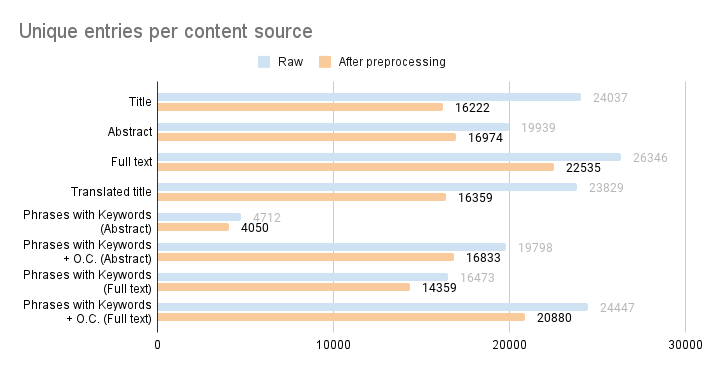
\includegraphics[width=0.75\textwidth]{Figures/05/Preprocessing_Unique entries per content source.png}
    \caption{Unique Entries per content source before and after preprocessing}
    \label{fig:05_unique_entries_after_preprocessing}
\end{figure}

\begin{table}[ht]
\centering
\resizebox{0.75\textwidth}{!}{
\begin{tabular}{|l|c|}
\hline
\textbf{Unique entries per \contentType{}} & \textbf{Percentage left} \\
\hline
\trafilaturaTitle{}                                 & 67.49\%          \\
\trafilaturaAbstract{}                              & 85.13\%          \\
\trafilaturaFulltext{}                              & 85.53\%          \\
\translationTitle{}                                 & 68.65\%          \\
\hline
\keyphrasesAbstractOnly{}                           & 85.95\%          \\
\keyphrasesAbstractOC{}                             & 85.02\%          \\
\keyphrasesFulltextOnly{}                           & 87.17\%          \\
\keyphrasesFulltextOC{}                             & 85.41\%          \\
\hline
\end{tabular}
}
\caption{Unique Entries per content source before and after preprocessing}
\label{tab:05_unique_entries_after_preprocessing}
\end{table}


Regarding the average token count of the content, the histograms in Figure \ref{fig:05_vsi_token_distribution_after_preprocessing} show that distributions across the four original \contentType{}s align with the original observations in Figure \ref{fig:04_vsi_token_distribution}. The same trend is observed for the \keyphrases{} as well. Upon comparing the means before and after preprocessing (Table \ref{tab:05_vsi_mean_tokens_before_after_preprocessing}), we observe that the means are higher for all the original content sources, except for the \trafilaturaFulltext{}.

The higher means can be attributed to the filtering of error messages, which tend to be short in length, and short entries that may correspond to scrapping errors. As for the \trafilaturaFulltext{}, upon closer inspection of the filtered-out \emph{long} texts identified as error messages, it was observed that they often pertain to topics such as website cookies or terms and conditions. These texts tend to be quite lengthy and are not typically found in website metadata (from where the \trafilaturaTitle{} and the \trafilaturaAbstract{} are extracted). This observation explains the lower mean for the \trafilaturaFulltext{} after preprocessing, which we interpret as a positive indication of our filtering approach.

When analyzing the \keyphrases{}, a significant decrease in the mean is noted, particularly for the \keyphrases{} extracted from the \trafilaturaFulltext{}. This reduction can be attributed to the fact that only a few sentences in an article usually contain the exact keywords used for locating them through a  Search Engine. Consequently, after preprocessing, the mean of the \keyphrases{} decreases substantially when compared to their original sources.

Overall, these observations highlight the effectiveness of our preprocessing in removing undesirable content while retaining relevant information.





\begin{figure}[ht]
    \centering
    \subfigure[\trafilaturaTitle{}]{
        \begin{adjustbox}{max height=0.18\textheight}
            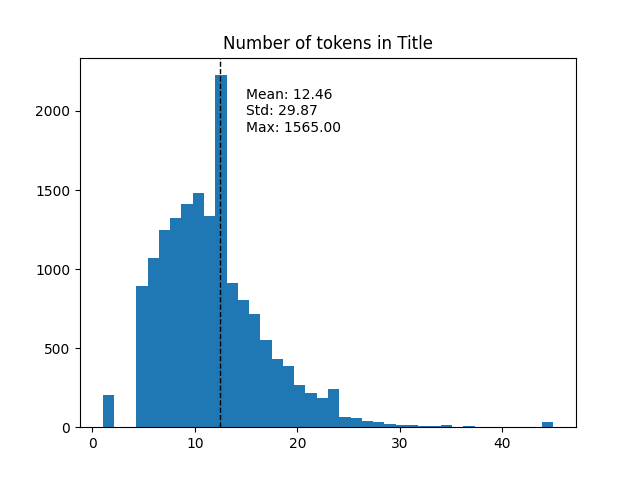
\includegraphics[width=0.45\textwidth]{Figures/05/Histograms/preprocessing length histogram parsed_trafilatura_title.png}
        \end{adjustbox}
        %\label{fig:image1}
    }
    \hfill
    \subfigure[\trafilaturaAbstract{}]{
            \begin{adjustbox}{max height=0.18\textheight}
            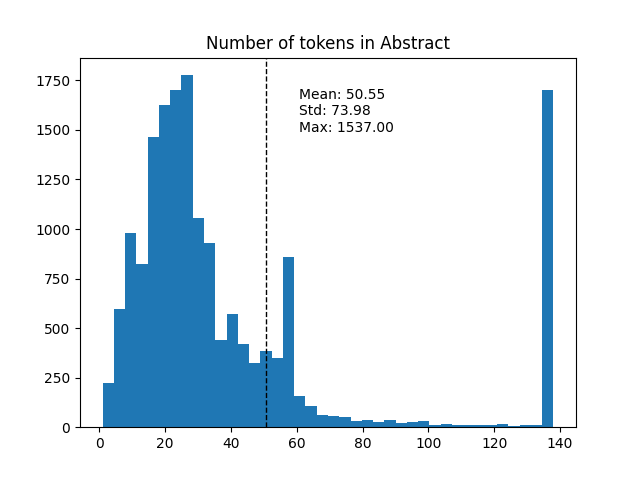
\includegraphics[width=0.45\textwidth]{Figures/05/Histograms/preprocessing length histogram parsed_trafilatura_abstract.png}
        \end{adjustbox}

        %\label{fig:image2}
    }
    
    \subfigure[\trafilaturaFulltext{}]{
        \begin{adjustbox}{max height=0.18\textheight}
          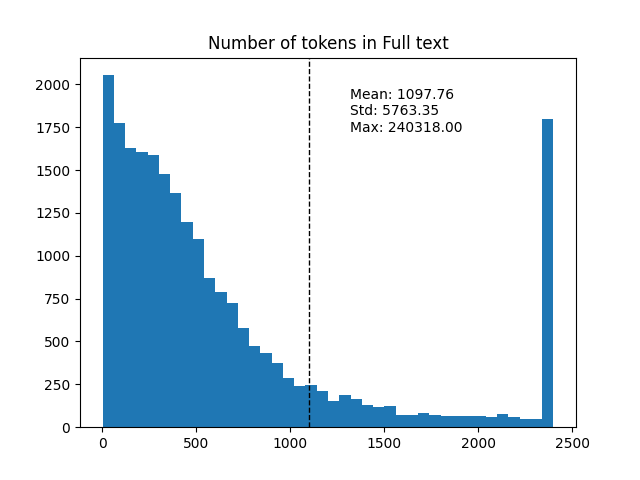
\includegraphics[width=0.45\textwidth]{Figures/05/Histograms/preprocessing length histogram parsed_trafilatura_fulltext.png}
        \end{adjustbox}
        %\label{fig:image3}
    }
    \hfill
    \subfigure[\translationTitle{}]{
            \begin{adjustbox}{max height=0.18\textheight}
                    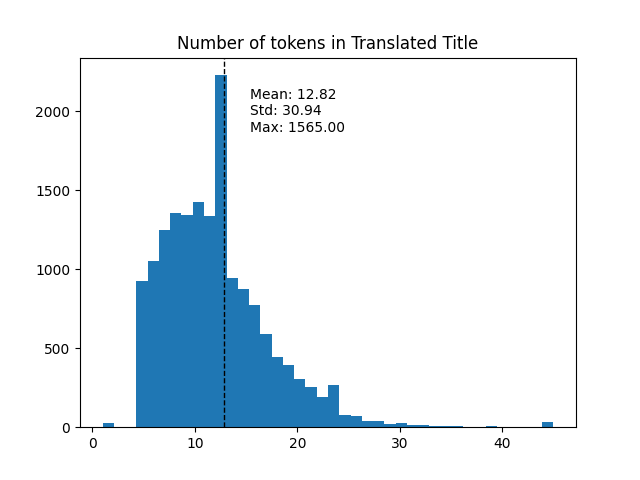
\includegraphics[width=0.45\textwidth]{Figures/05/Histograms/preprocessing length histogram translation_title.png}
        \end{adjustbox}
        %\label{fig:image4}
    }
    
    
    %%
    \subfigure[\keyphrasesAbstractOnly{}]{
        \begin{adjustbox}{max height=0.18\textheight}
            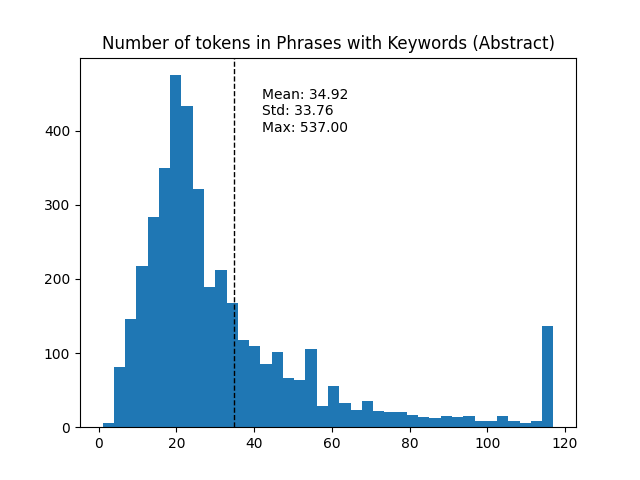
\includegraphics[width=0.45\textwidth]{Figures/05/Histograms/preprocessing length histogram sentence_with_keywords_parsed_trafilatura_abstract_only_relevant_sentences.png}
        \end{adjustbox}
        
        %\label{fig:image2}
    }
    \hfill
    \subfigure[\keyphrasesAbstractOC{}]{
         \begin{adjustbox}{max height=0.18\textheight}
         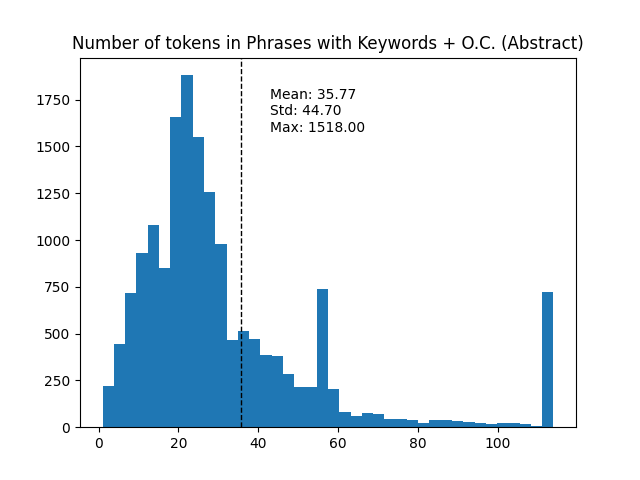
\includegraphics[width=0.45\textwidth]{Figures/05/Histograms/preprocessing length histogram sentence_with_keywords_parsed_trafilatura_abstract_keep_original_content.png}
        \end{adjustbox}
    
        %\label{fig:image1}
    }

    
    \subfigure[\keyphrasesFulltextOnly{}]{

    \begin{adjustbox}{max height=0.18\textheight}
           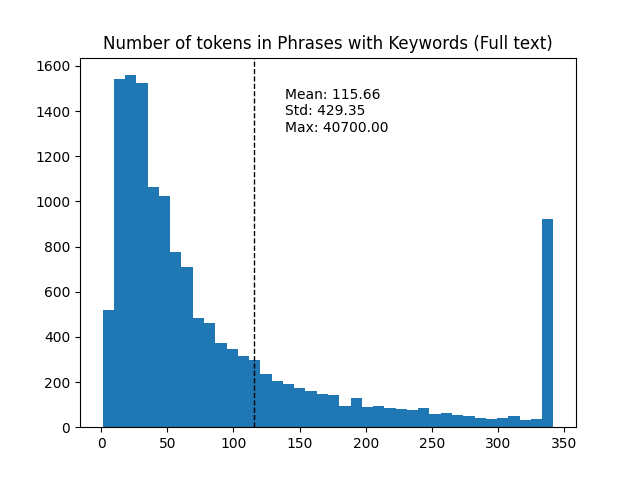
\includegraphics[width=0.45\textwidth]{Figures/05/Histograms/preprocessing length histogram sentence_with_keywords_parsed_trafilatura_fulltext_only_relevant_sentences.png}
        \end{adjustbox}
    
        %\label{fig:image4}
    }
    \hfill
        \subfigure[\keyphrasesFulltextOC{}]{
        \begin{adjustbox}{max height=0.18\textheight}
            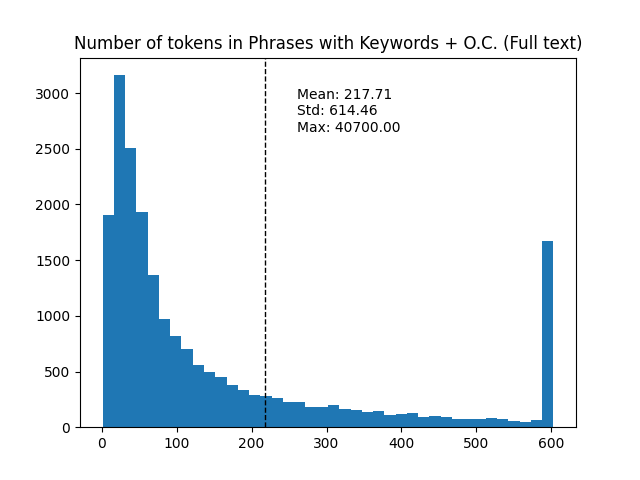
\includegraphics[width=0.45\textwidth]{Figures/05/Histograms/preprocessing length histogram sentence_with_keywords_parsed_trafilatura_fulltext_keep_original_content.png}
        \end{adjustbox}
        
        %\label{fig:image3}
    }

    
    \caption{
    Length (in n. of tokens) of the \contentType{}s in the \VSI{} dataset after preprocessing}
    \label{fig:05_vsi_token_distribution_after_preprocessing}
\end{figure}





\begin{table}[ht]
\centering
\resizebox{\textwidth}{!}{
\begin{tabular}{|l|c|c|}
\hline
\textbf{\contentType{}} & \textbf{Before preprocessing} & \textbf{After preprocessing} \\
\hline
\trafilaturaTitle{} & 11.29  & 12.46 \\
\trafilaturaAbstract{}  & 50.02     & 50.55     \\
\trafilaturaFulltext{}    & \textcolor{orange}{1102.29}     & \textcolor{orange}{1097.76}    \\
\translationTitle{}   & 11.66     & 12.82     \\ \hline
\keyphrasesAbstractOnly{}  & (50.02)     & 34.92     \\
\keyphrasesAbstractOC{} & (50.02)     & 35.77     \\

\keyphrasesFulltextOnly{} & (1102.29)     & 115.66    \\
\keyphrasesFulltextOC{} & (1102.29)     & 217.71    \\

\hline
\end{tabular}
}
\caption{Mean token counts before and after preprocessing the \VSI{} dataset}
\label{tab:05_vsi_mean_tokens_before_after_preprocessing}
\end{table}


\putInBox{
By applying our preprocessing approach, we construct eight labelled datasets for binary \textclassification{} (Figure \ref{fig:05_vsi_pos_neg_balance}). These datasets exhibit a balance of positives and negatives ranging from 12 to 14\% positives, and from 86 to 88\% negatives\footnote{For more details, see Table \ref{appendix03:tab:vsi_positive_negative_balance} in \appendixname{} \ref{appendix03:preprocessing_statistics}}, representing a slight improvement compared to the original dataset, which had a balance of 10\% positives to 90\% negatives (Figure \ref{fig:04_naive_positives_and_negatives}). 
}

The only exception are the \keyphrases{} from the \trafilaturaAbstract{} discarding Original Content (``\keyphrasesAbstractOnly{}"). This specific dataset displays a 27\% positive and 73\% negative balance. The reasons behind this imbalance can be attributed to the factors previously explained. As the metadata required for extracting the \trafilaturaAbstract{} may be empty or uninformative; and few entries may contain the exact search keywords we are looking for; the dataset is substantially reduced, resulting in only 4,050 unique entries for the \keyphrasesAbstractOnly{}  as opposed to the original 19,939  unique entries for the \trafilaturaAbstract{} ($\approx$ 20\% left). Consequently, the significantly smaller dataset size has led to a noticeable change in the balance of the labels.


\begin{figure}[ht]
    \centering
    \subfigure[\trafilaturaTitle{}]{
        \begin{adjustbox}{max height=0.18\textheight}
            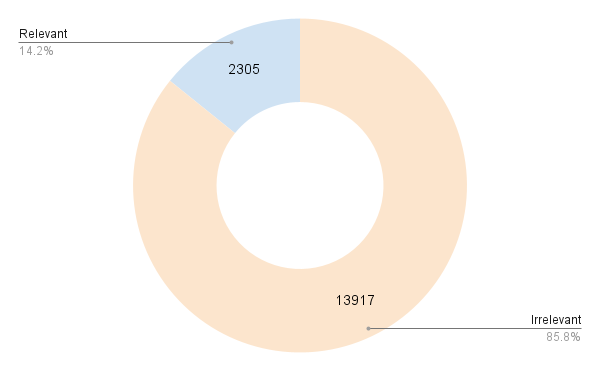
\includegraphics[width=0.45\textwidth]{Figures/05/Charts/balance Title.png}
        \end{adjustbox}
        
        %\label{fig:image1}
    }
    \hfill
    \subfigure[\trafilaturaAbstract{}]{
        \begin{adjustbox}{max height=0.18\textheight}
            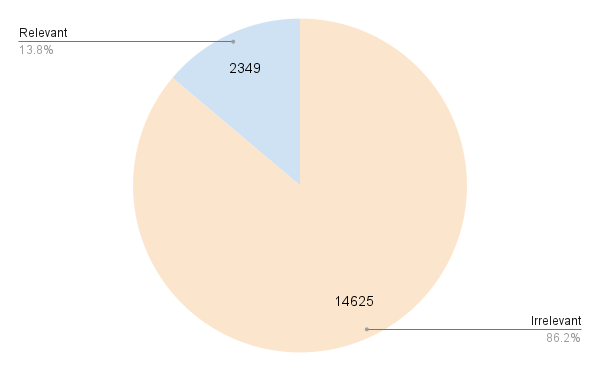
\includegraphics[width=0.45\textwidth]{Figures/05/Charts/balance Abstract.png}
        \end{adjustbox}
        
        %\label{fig:image2}
    }
    
    \subfigure[\trafilaturaFulltext{}]{
        \begin{adjustbox}{max height=0.18\textheight}
            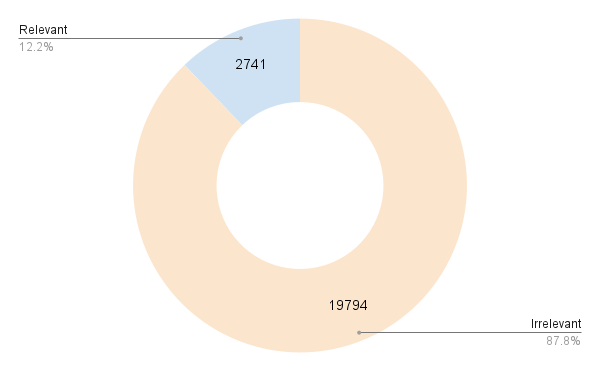
\includegraphics[width=0.45\textwidth]{Figures/05/Charts/balance Fulltext.png}
        \end{adjustbox}
        
        %\label{fig:image3}
    }
    \hfill
    \subfigure[\translationTitle{}]{
        \begin{adjustbox}{max height=0.18\textheight}
            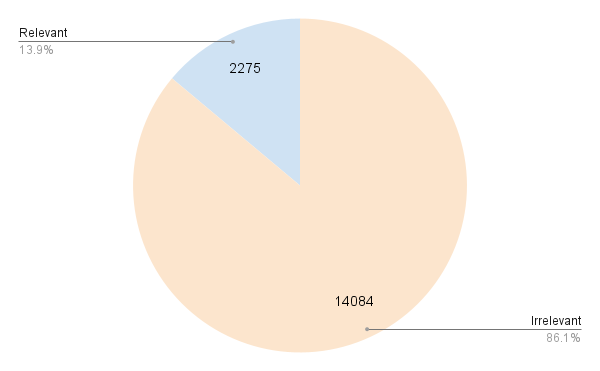
\includegraphics[width=0.45\textwidth]{Figures/05/Charts/balance Translated Title.png}
        \end{adjustbox}
        %\label{fig:image4}
    }
    
    
    %%
    \subfigure[\keyphrasesAbstractOnly{}]{
        \begin{adjustbox}{max height=0.18\textheight}
            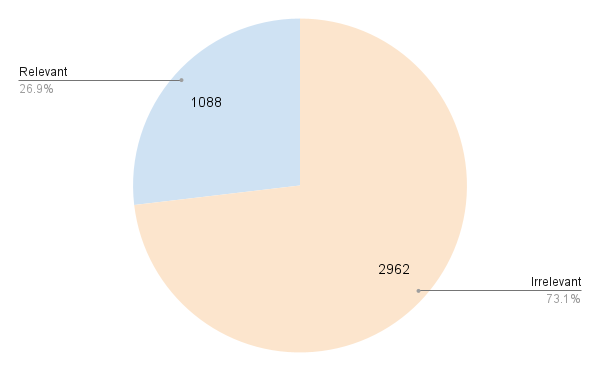
\includegraphics[width=0.45\textwidth]{Figures/05/Charts/balance Sentence with Keywords Abstract.png}
        \end{adjustbox}
        %\label{fig:image2}
    }
    \hfill
    \subfigure[\keyphrasesAbstractOC{}]{
        \begin{adjustbox}{max height=0.18\textheight}
            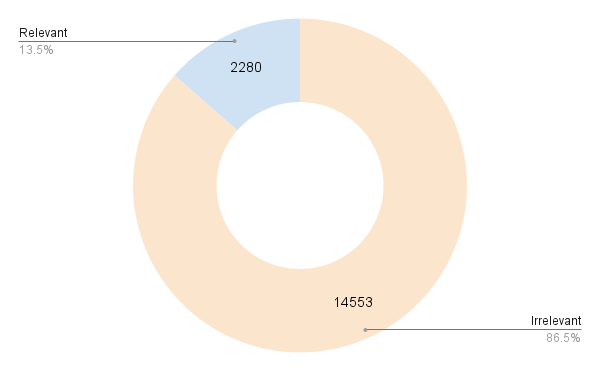
\includegraphics[width=0.45\textwidth]{Figures/05/Charts/balance Sentece with Keywords and OC Abstract.png}
        \end{adjustbox}
        %\label{fig:image1}
    }

    
    \subfigure[\keyphrasesFulltextOnly{}]{
        \begin{adjustbox}{max height=0.18\textheight}
            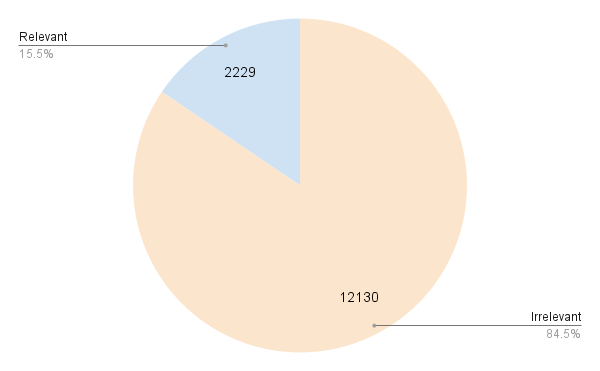
\includegraphics[width=0.45\textwidth]{Figures/05/Charts/balance Sentence with keywords Fulltext.png}
        \end{adjustbox}
        %\label{fig:image4}
    }
    \hfill
    \subfigure[\keyphrasesFulltextOC{}]{
        \begin{adjustbox}{max height=0.18\textheight}
            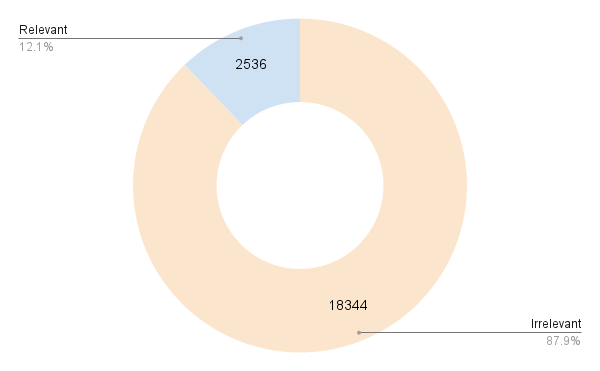
\includegraphics[width=0.45\textwidth]{Figures/05/Charts/balance Sentence with keywords and OC Fulltext.png}
        \end{adjustbox}
        %\label{fig:image3}
    }

    
    \caption{Positive/Negative balance after preprocessing the \VSI{} dataset}
    \label{fig:05_vsi_pos_neg_balance}
\end{figure}




% making sure to print all tables and figures 
\clearpage